\section{Measuring TritonSort's Energy Efficiency}

A potential benefit of improved per-node efficiency is lower the amount of
energy required to complete a given task. In this section, we describe a
quantitative study of TritonSort's memory usage performed while measuring
TritonSort's performance for the JouleSort benchmark. JouleSort measures the
energy efficiency of a large-scale sort, and its evaluation metric is ``records
sorted per Joule.''

When measuring the energy consumed by the testbed during the run, we measure
the combined energy used by the experiment nodes, the experiment head node, and
the 10Gbps switch that connects the machines together. We present JouleSort
measurements for both TritonSort and an early prototype of Themis, the final
implementation of which is described in Chapter~\ref{chapter:themis}.

\subsection{Measuring the Switch}
To measure the energy used by our Cisco 5596UP datacenter switch, we plugged the
switch into an Avocent PM 3000V PDU during our sorting runs. The PDU tracks
maximum, minimum and ``present'' power draw on a per-port basis. To determine
the total amount of energy used by the switch throughout the run, we multiplied
the maximum power draw from the switch (in watts) as measured by the PDU by the
duration of the run in seconds. This overestimates the energy used by the
switch, but makes our calculations easier. The power drawn by the switch
measured in this way is 566 watts.

\subsection{Measuring the Nodes}
We measured the power consumed by the cluster machines (both experimental nodes
and head node) using two different power meters. The first meter is available
on each machine, but does not meet the accuracy standards required by the
sort benchmark's guidelines. The second can only be attached to one machine at a
time, but meets the required accuracy standards. As we will show in later
sections, the two meters' power measurements are very similar. We describe each
meter and the methodology for measuring power from it below.

One danger when measuring power on many machines is that the clocks on those
machines may become out of sync and cause the aggregate power measurements
from multiple nodes (that should be correlated by time but aren't) to be
inaccurate. To prevent this from being a problem, we issue all power meter
queries from a single machine and timestamp the power meter measurements when
they are received. Further, we issue the measurements from the experiment head
node so that the timestamps recorded when the sort starts and stops (see above)
are taken from the same clock as the timestamps for the power measurements.

All power measurements are performed by simple Python scripts. The content of
the script varies depending on the power monitoring system being queried. In
cases where multiple machines are to be monitored at once, the script spawns a
thread per monitored machine and each thread runs independently. We start the
power monitor scripts manually several minutes before starting the sort run to
allow them to ``warm up'' and make sure everything is working properly, and
stop them manually several minutes after the sort run ends. The scripts dump
power measurements to a file as they run, and these files are analyzed after
the run to determine total energy usage.

\subsubsection{HP ILO Power Meters}

The first meter we used was the power measurement subsystem of HP's Integrated
Lights-Out (ILO) management tool. Each of our DL380G6 machines comes equipped
with an on-board service processor running version 1.82 of ILO2.

We query the ILO power meter using the Remote Board Insight Command Language
(RIBCL). RIBCL allows operators to issue commands to ILO by sending an XML
document to the ILO system over an SSL-encrypted TCP session and receive an
XML response. The power monitoring script repeatedly opens an SSL connection to
the ILO system, issues a power monitoring command, retrieves a response, and
closes the connection.

RIBCL's power measurement reports four numbers: maximum, minimum and average
power over the past 24 hours, and ``present'' power, which measures the number
of watts for the most recent 0.5 second sample. We use present power as our
power measurement for each sample.

Unfortunately, RIBCL requires that only a single XML document ``command'' be
sent per connection. We found in practice that we could not reliably issue
RIBCL commands to the ILO system more than once every 15 seconds because the
on-board service processor is quite slow and the high overhead of establishing
an SSL session must be incurred once per measurement.

\subsubsection{WattsUp? Power Meter}

To provide once-per-second measurements of our machines' power consumption, we
attached a power meter that could provide once-per-second power measurements to
a representative node in the cluster. The particular meter that we used was the
IEC 320 universal outlet (UO) version of the WattsUp? Pro/ES/.Net
power monitor. We refer to this meter as the WattsUp meter for brevity for the
remainder of the text. We chose this meter because of its ready availability
and known reliability; several other research projects at UCSD have used this
meter to measure server power successfully.

The WattsUp meter has a simple serial-over-USB interface. The client opens a
TCP connection to the meter and sends the meter a request for data and a data
collection interval. The meter responds by sending the requested data once per
interval until it's told to stop or the client closes the TCP connection. Our
power measurement script sends the meter a request for power information at an
interval of one second. The script then receives and parses the response (by
issuing a blocking read call to the socket, which consistently unblocks with a
new response once per second) and appends the parsed response to a file.

During the first four runs of each benchmark type, we used the WattsUp meter to
measure the power on a random experiment node. On the fifth run, we used it to
measure the experimental head node. Since the head node is not doing anything
particularly intensive (monitoring power on each machine and recording
experiment time), we found that its power consumption was relatively
low. Through measurements on both types of power meters, we found that the
average draw for the head node was 134 watts with a deviation of about 2
watts. Because of this, we assume that the experiment head node's power draw is
a constant 134 watts for the duration of the sort run.

\subsubsection{Resolving Discrepancies Between Meters}

\begin{figure}
\centering
\begin{subfigure}[b]{\columnwidth}
  \centering
  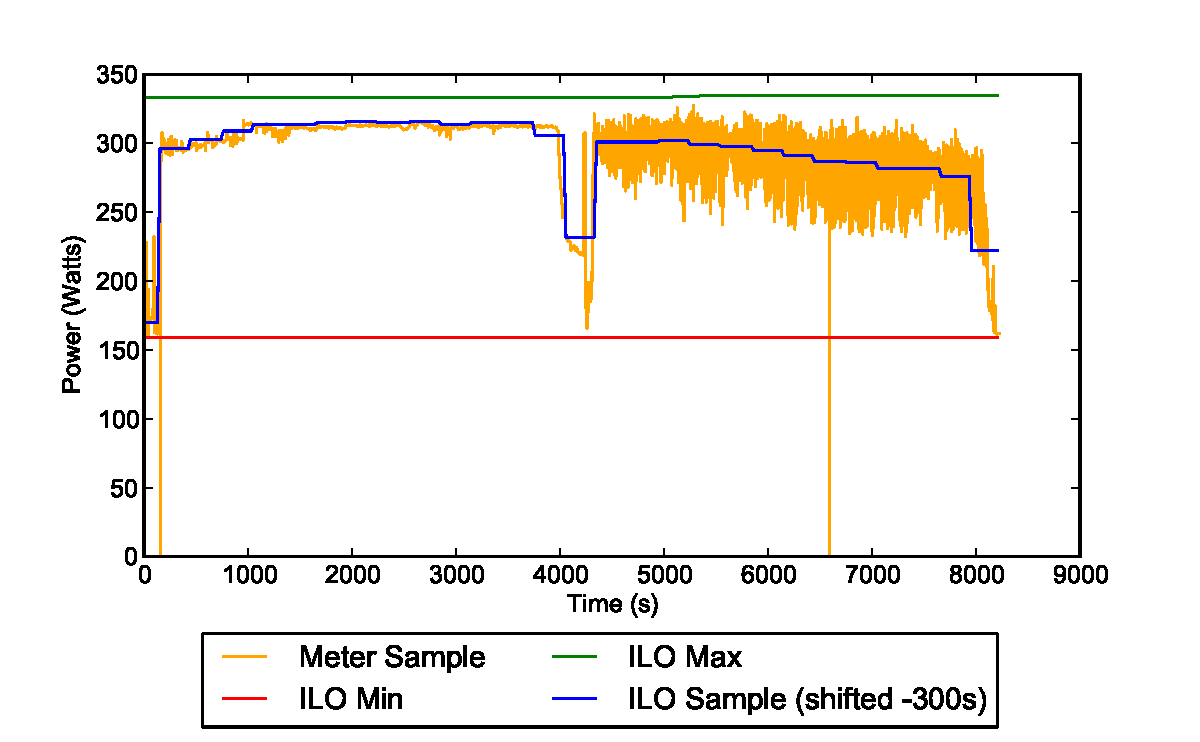
\includegraphics[width=\columnwidth]{tritonsort/graphs/joulesort_raw.pdf}
  \caption{\label{fig:power:raw} Raw WattsUp meter data}
\end{subfigure}
\begin{subfigure}[b]{\columnwidth}
  \centering
  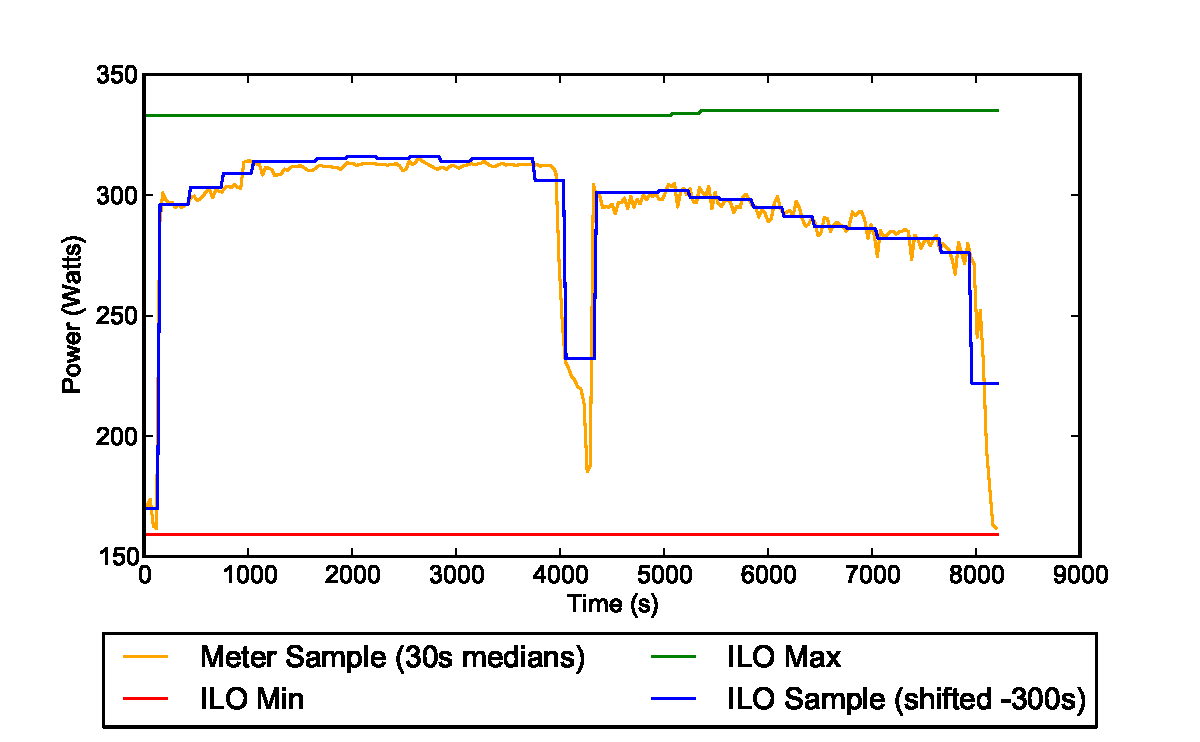
\includegraphics[width=\columnwidth]{tritonsort/graphs/joulesort_30s.pdf}
  \caption{\label{fig:power:30s} Median of each 30 seconds of WattsUp data}
\end{subfigure}
\caption{\label{fig:power} Power consumed by a representative node during a
  JouleSort run, comparing the results of the two power meters used.}
\end{figure}

We found that the power measured by the ILO system lags that measured by the
WattsUp meter by exactly five minutes. Figure~\ref{fig:power} shows both the
maximum, minimum and ``present'' power reported by the ILO and the power
reported by the WattsUp meter during a JouleSort run, with the ILO
measurements appropriately time-shifted. When calculating power with the ILO
meters, we time-shifted all samples by 5 minutes to compensate for this
observation and allowed the power collection scripts to run for several minutes
after the sort run finished to collect sufficient additional samples to cover
the entirety of the sort run.

In these runs you can see that there is a sharp reduction in power usage about
halfway through the sort run.  This is a result of the barrier between phases
one and two.  Due to the natural variation in node performance, some nodes
finish phase one earlier than others, and so their power usage is reduced.
However, none of the nodes can start phase two until all nodes are done with
phase one, which results in the gap visible in Figure~\ref{fig:power}.

The WattsUp meter's data is more variable during phase two; we suspect that
this is due to the fact that the CPU is far more active during phase two than
it is during the other phases. However, if we look at the median power reported
by the WattsUp meter during each 30 second interval throughout the run, we
notice that the WattsUp meter's measurements track the ILO's measurements quite
closely.


\subsection{Calculating Energy}

To estimate energy used by the experiment head node and the switch, we
multiply their estimated instantaneous power draws (134 watts and 566 watts,
respectively) by the duration of the sort run in seconds. Call the energy
used by the head node and the switch $E_{head}$ and $E_{switch}$ respectively.

All power measurements reported by our meters are reported in watts. To obtain
an energy measurement from this collection of instantaneous power measurements,
we start by filtering the set of measurements so that we only consider those
measurements that were taken on or after the sort run's start timestamp and on
or before the sort run's end timestamp. The subsequent power calculation varies
depending on the meter being used. We refer to the energy used by the
experiment nodes as $E_{nodes}$.

When calculating power based on measurements gathered from the ILO meters, we
start by sorting measurements in ascending order by timestamp. We then compute
the total energy for a node in the following way. For each measurement $(W_i,
T_i)$, we consider the previous measurement $(W_{i-1}, T_{i-1})$ and add $W_i *
(T_i - T_{i-1})$ to the total energy. In cases where the measurement abuts the
start or end of the run, we use the start and end timestamps of the sort run as
$T_i$ and $T_{i - 1}$ as appropriate to ``fill in the gaps'' at the beginning
and end of the run. We compute the total energy for each node in this way and
sum the energy from each node to compute $E_{nodes}$.

\begin{table}
\centering
\caption{\label{table:power_draw} Average power consumed by a node throughout
a sort benchmark run for the first four trials of our JouleSort experiments}
\begin{tabular}{|cc|c|}
\hline
\textbf{System} & \textbf{Trial} & \textbf{Avg. Server Power} \\
\hline
TritonSort & 1 & 287 Watts \\
TritonSort & 2 & 285 Watts \\
TritonSort & 3 & 309 Watts \\
TritonSort & 4 & 297 Watts \\
Themis Prototype & 1 & 290 Watts \\
Themis Prototype & 2 & 285 Watts \\
Themis Prototype & 3 & 293 Watts \\
Themis Prototype & 4 & 306 Watts \\
\hline
\end{tabular}
\end{table}

When using the WattsUp meter, we have once-per-second measurements and can
produce power estimates in line with the sort benchmark guidelines. To do this,
we compute that average (mean) power for the representative node. For the first
four trials (where an experimental node is being measured), this data is
derived by taking the average of all measurements taken from the WattsUp meter
during the sort run. For the fifth trial (where the head node is being
measured), the average power is assumed to be the average of the previous four
trials.

We believe that this assumption is reasonable because the average power
consumed by a node does not vary much; we provide the average power drawn by a
node in the first four trials in Table~\ref{table:power_draw}. The standard
deviation for the first four measurements is 11 watts for TritonSort and 9 watts
for the early Themis prototype, 3.7\% and 3.0\% of the mean, respectively.

Once we have computed the average power for a representative node, we multiply
that average power by the length of the run in seconds to yield the total energy
consumption for a node, and multiply that number by the number of nodes (52 in
our experiments) to yield $E_{nodes}$.

Once we have computed $E_{nodes}$, $E_{head}$ and $E_{switch}$, we compute
total energy $E_{tot}$ as $E_{nodes} + E_{head} + E_{switch}$.

\subsection{Measurement Results}

\begin{table}
\centering
\caption{\label{table:raw_energy} Total energy measured for each 100TB trial by
  both WattsUp and ILO meters}
\begin{tabular}[t]{|c|c|cc|cc|}
\hline
 &  & \multicolumn{2}{c|}{\textbf{Energy (Joules)}} & \multicolumn{2}{c|}{\textbf{Records
per Joule}}\\
\textbf{Benchmark} & \textbf{Trial} & WattsUp & ILO & WattsUp & ILO\\
\hline
TritonSort & 1 & 103,180,896 & 108,054,648 & 9,692 & 9,255 \\
TritonSort & 2 & 99,312,480 & 105,333,939 & 10,069 & 9,494 \\
TritonSort & 3 & 109,495,040 & 105,425,639 & 9,133 & 9,485 \\
TritonSort & 4 & 102,724,272 & 105,523,992 & 9,735 & 9,477 \\
TritonSort & 5 & 101,108,112 & 103,656,684 & 9,890 & 9,647 \\
\hline
\hline
Themis Prototype & 1 & 129,774,720 & 136,098,976 & 7,706 & 7,348 \\
Themis Prototype & 2 & 127,434,720 & 135,998,793 & 7,847 & 7,353 \\
Themis Prototype & 3 & 132,077,568 & 136,851,456 & 7,571 & 7,307 \\
Themis Prototype & 4 & 137,082,224 & 136,259,721 & 7,295 & 7,339 \\
Themis Prototype & 5 & 132,380,352 & 135,332,800 & 7,554 & 7,389 \\
\hline
\end{tabular}
\end{table}

\begin{table}
\centering
\caption{\label{table:energy_stats} Statistics for the energy measurements
  presented in Table~\ref{table:raw_energy}}
\resizebox{\columnwidth}{!}{
\begin{tabular}[t]{|cc|cccc|}
\hline & & \multicolumn{4}{c|}{\textbf{Energy (Joules)}} \\
\textbf{Benchmark} & \textbf{Meter} & Median & Mean (Average) & Std. Dev. &
Std. Err\\
\hline
TritonSort & ILO & 105,425,639 & 105,598,980 & 3,170,018 & 1,417,675 \\
TritonSort & WattsUp & 102,724,272 & 103,164,160 & 736,610 & 329,422 \\
Themis Prototype & ILO & 136,098,976 & 136,108,349 & 4,086,316 & 1,827,456 \\
Themis Prototype & WattsUp & 132,077,568 & 131,749,917 & 941,356 & 420,987 \\
\hline
\end{tabular}
}
\end{table}

We ran five trials each of a 100TB sort in both TritonSort and the Themis
prototype. The raw energy measurements for these trials are given in
Table~\ref{table:raw_energy} and statistics concerning the total energy
measurements are given in Table \ref{table:energy_stats}. TritonSort sorted an
average of 9,704 records per Joule. The Themis Prototype sorted an average of
7,595 records per Joule.


\subsubsection{Deriving Standard Deviation and Standard Error}

When calculating standard deviation and standard error in Table
\ref{table:energy_stats}, we assume that the WattsUp meters are accurate to
\textpm 2\% and the ILO meters are accurate to \textpm 10\%. We were unable to
obtain any data about the accuracy of Avocent's PDUs, and so we assume somewhat
pessimistically that the PDUs are accurate to \textpm 5\%.

We obtained standard deviation in the following way. First, we derived the mean
power drawn by each server, the head node, and the switch. When using the
WattsUp meter's measurements, we simply used the mean of all power measurements
logged by the meter. When using the ILO meter's measurements, we derived the
mean power draw for a node by dividing the total amount of energy consumed by
the node by the trial's runtime. Call the mean power produced by server $X$
$P_{N_X}$, the mean power produced by the head node $P_H$ and the mean power
produced by the switch $P_S$.

We then multiplied each mean power value by its respective meter's accuracy to
yield the uncertainty $U(P_{N_X})$, $U(P_{H})$ and $U(P_{S})$ of each power
measurement. We then multiplied these uncertainties by the trial runtime to
yield the uncertainty $U(E_{N_X})$, $U(E_{H})$ and $U(E_{S})$ of each energy
measurement. Once these values were derived, we used error propagation to yield
the total energy measurement uncertainty for the trial using the following
formula:

\[U(E_{trial}) = \sqrt{(\sum_{X=0}^{51}{U(E_{N_X})^2}) + U(E_H)^2 + U(E_S)^2}\]

Once $U(E_{trial})$ was calculated for each trial, we performed a further round
of error propagation across trials to yield total uncertainty, i.e. standard
deviation.

\[U(E_{total}) = \sqrt{\sum_{T=1}^{5}{U(E_{trial T})^2}}\]

Standard error is derived by dividing standard deviation by $\sqrt{5}$.
